\documentclass[11pt,a4paper,sans]{moderncv}
\usepackage[T2A]{fontenc}
\usepackage[utf8]{inputenc}
\usepackage[english, russian]{babel}
\usepackage{cmap}
\usepackage{pscyr}

\moderncvstyle{classic}
\moderncvcolor{blue}

\usepackage[scale=0.75, top=0.5in, bottom=1in,left=0.8in,right=0.65in]{geometry}
\setlength{\hintscolumnwidth}{3.35cm}
\graphicspath{{../img/icons/}}

\nopagenumbers
\widowpenalty=0

\firstname{Андрей}
\familyname{Акиньшин}

%\title{.NET-разработчик}
\mobile{+7-913-240-02-04}
\email{andrey.akinshin@gmail.com}
\homepage{aakinshin.net}{aakinshin.net}
\photo[70pt][0.4pt]{./photo}

%----------------------------------------------------------------------------------------

\begin{document}

\makecvtitle

\section{Программирование}
\cvitem{}{\myemph{Microsoft .NET MVP (2015), Lead .NET Developer}}
\cvitem{Основные навыки}{.NET/C\#, R, Алгоритмы, Математика, Проектирование архитектуры}

\cvitem{09/2010--Сейчас}{
    
\includegraphics[height=12px]{perpetuum}
    \myhref{http://www.perpetuumsoft.com/}{{Perpetuum Software LLC}} / 
    
\includegraphics[height=12px]{enterra}
    \myhref{http://www.enterra.ru/}{{Энтерра Софт}} / 
    
\includegraphics[height=12px]{notariat}
    \myhref{http://notariatsoft.ru/}{{Адаптивные технологии}}
    \newline
    \phantom{~~~~}
    \mbox{
        \begin{tabular}{ll}
            09/2010--08/2011     & \myemph{Стажёр}\\
            09/2011--01/2013     & \myemph{Программист}\\
            02/2013--Сейчас~~~~~ & \myemph{Ведущий программист}\\
        \end{tabular}
    }
}
\cvitem{}{
    \pseudoitem
    
\includegraphics[height=12px]{pv}
    \myhref{http://passportvision.ru/}{PassportVision}:
    Программа для распознавания паспортов.\newline
    Ведущий разработчик, ответственен за архитектуру и алгоритмы. 
}
\cvitem{}{
    \pseudoitem
    
\includegraphics[height=12px]{grapholite}
    \myhref{http://grapholite.com/}{Grapholite}: 
    Редактор диаграмм под 
    \myhref{http://apps.microsoft.com/windows/app/grapholite-diagrams-pro/99164828-b985-44ad-af71-58827d8d8a13}{
\includegraphics[height=12px]{windows8}}
    \myhref{http://www.windowsphone.com/en-us/store/app/grapholite-diagrams-phone-edition/4e89fe82-db21-45c5-a284-8de9a443fb70}{
\includegraphics[height=12px]{winphone}}
    \myhref{https://grapholite.com/Download/Grapholite.msi}{
\includegraphics[height=12px]{wpf}}
    \myhref{https://grapholite.com/Designer}{
\includegraphics[height=12px]{silverlight}}
    \myhref{https://itunes.apple.com/us/app/grapholite-diagrams-flow-charts/id954302708?ls=1&mt=8}{
\includegraphics[height=12px]{ios}}
    \myhref{https://play.google.com/store/apps/details?id=com.grapholite.diagramsdemo}{
\includegraphics[height=12px]{android}}  	  
    (аналог MS~Visio). 
    Ответственен за алгоритмы, математику и часть архитектуры.
}
\cvitem{}{
    \pseudoitem
    
\includegraphics[height=12px]{knockout-mvc}
    \myhref{http://knockoutmvc.com/}{Knockout MVC}:~
    ASP.NET MVC-обёртка для knockout.js.\newline
    Главный разработчик: архитектура, API, основная логика, вёрстка и~т. д.
}
\cvitem{}{
    \pseudoitem
    
\includegraphics[height=12px]{ui-controls}
    \myhref{http://www.perpetuumsoft.com/Windows8-UI-Controls.aspx}{UI Controls for Windows 8}: 
    Набор контролов под Windows 8.\newline
    Главный разработчик: архитектура, API, XAML, демо-проект и~т.~д. 
}

\section{Научная деятельность}
\cvitem{}{\myemph{Кандидат физико-математических наук (05.13.18), Постдок}}
\cvitem{08/2012--Сейчас}{
    
\includegraphics[height=12px]{math-nsc}
	\myhref{http://www.math.nsc.ru/}{ИМ СО РАН}, \myhref{http://a-server.math.nsc.ru/IM/lbrt.asp?CodLB=59}{лаб. обратных задач мат. физики} (Новосибирск)
     \newline
     \phantom{~~~~}
     \mbox{
         \begin{tabular}{ll}
             08/2012--06/2014     & \myemph{Инженер}\\
             07/2014--Сейчас~~~~~ & \myemph{Научный сотрудник}\\
            \end{tabular}
        }
}

\cvitem{}{	
	Области исследования: биоинформатика, генные сети, теория бифуркаций.\newline
	Гранты: \myhref{http://www.rfbr.ru/rffi/ru/contests_results2012/o_64737}{РФФИ 12-01-00074}, РФФИ 15-01-00745 А. 	
}
\cvitem{10/2014--Сейчас}{
    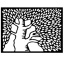
\includegraphics[height=12px]{weizmann}
	\myhref{http://www.weizmann.ac.il/}{Институт Вейцмана}, \myhref{http://wws.weizmann.ac.il/math/}{Кафедра математики} (Израиль, Реховот)
     \newline
     \phantom{~~~~}
     \mbox{
         \begin{tabular}{ll}
             10/2014--Сейчас~~~~~ & \myemph{Postdoctoral Research Fellow}\\
            \end{tabular}
        }
}
\cvitem{}{	
	Области исследования: цифровая обработка сигналов, преобразование Фурье.
}

\section{Олимпиады}
\cvitem{}{
	
\includegraphics[height=12px]{neerc}
	Всероссийская олимпиада школьников по информатике \myhref{http://neerc.ifmo.ru/school/archive/2005-2006/ru-olymp-roi-2006-standings.html}{РОИ 2006}:
	\myemph{Золото}
}
\cvitem{}{
	
\includegraphics[height=12px]{acm-icpc}  
	Чемпионат мира по программированию \myhref{http://icpc.baylor.edu/community/results-2008}{ACM ICPC 2008}:
	\myemph{Сертификация}
}
\cvitem{}{
	
\includegraphics[height=12px]{acm-icpc}
	Чемпионат мира по программированию \myhref{http://icpc.baylor.edu/community/results-2009}{ACM ICPC 2009}:
	\myemph{Серебо}
}


\section{Преподавание}
\cvitem{09/2006--05/2012}{
	
\includegraphics[height=12px]{s42}
	\myemph{Тренер сборной} 
	по программированию в \myhref{http://s42.asu.ru/}{МБОУ <<Гимназия №42>>} г. Барнаула.}
\cvitem{09/2009--06/2012}{
  
\includegraphics[height=12px]{aeli}
  \myemph{Преподаватель} информатики в Алтайском Экономико-Юридическом Институте.}
\cvitem{09/2011–-11/2011}{
  
\includegraphics[height=12px]{ministry}
  \myemph{Преподаватель} 
  в рамках федеральной программы \myhref{http://miptic.ru/nir/podgotovka.html}{Ф-263 №4}.
 }

\section{Избранные open source проекты}
\cvitem{\myhref{https://github.com/AndreyAkinshin/ProblemBook.NET}{Задачник.NET}}{
	 Online-книга с подборкой задач по .NET/C\#
}
\cvitem{\myhref{https://github.com/AndreyAkinshin/Russian-Phd-LaTeX-Dissertation-Template}{Phd-LaTeX-Template}}{
	\LaTeX-шаблон для русской кандидатской диссертации
}
\cvitem{\myhref{https://github.com/AndreyAkinshin/BenchmarkDotNet}{BenchmarkDotNet}}{
	Библиотека для создания бенчмарков под .NET 
}
\cvitem{\myhref{https://github.com/AndreyAkinshin/InteropDotNet}{InteropDotNet}}{
	Реализация кроссплатформенного AnyCPU P/Invoke под .NET
}
\cvitem{\myhref{https://github.com/AndreyAkinshin/CultureInfoExplorer}{CultureInfoExplorer}}{
	WPF-обозраватель различных CultureInfo в .NET 
}

\section{Избранные выступления}
\cvitem{\myhref{http://msk2014.dotnext.ru/}{.NEXT 2014 Moscow}}{
    <<Поговорим о различных версиях .NET>>
}
\cvitem{\myhref{http://spb2015.dotnext.ru/}{.NEXT 2015 Piter}}{
    <<Поговорим о микрооптимизациях .NET-приложений>>
}
\cvitem{\myhref{http://dotnetconf.ru/}{.dotnetconf 10}}{
    <<Практические приёмы оптимизации .NET-приложений>>
}
\cvitem{\myhref{http://dotnetconf.ru/}{CLRium \#2}}{    
    <<CoreCLR, RyuJIT и DNX>>
}

\section{Изобранные сертификаты}
\cvitem{07/2014}{
	\myhref{http://aakinshin.ru/content/cert/mcp.pdf}{Microsoft Certified Professional (MCP)}
}
\cvitem{12/2014}{
	\myhref{https://www.coursera.org/account/accomplishments/specialization/44Y2uInkEe}{The Data Science Specialization, 10 курсов [Coursera]}
}
  
\section{Профили}
\cvitem{Резюме и блог}{
    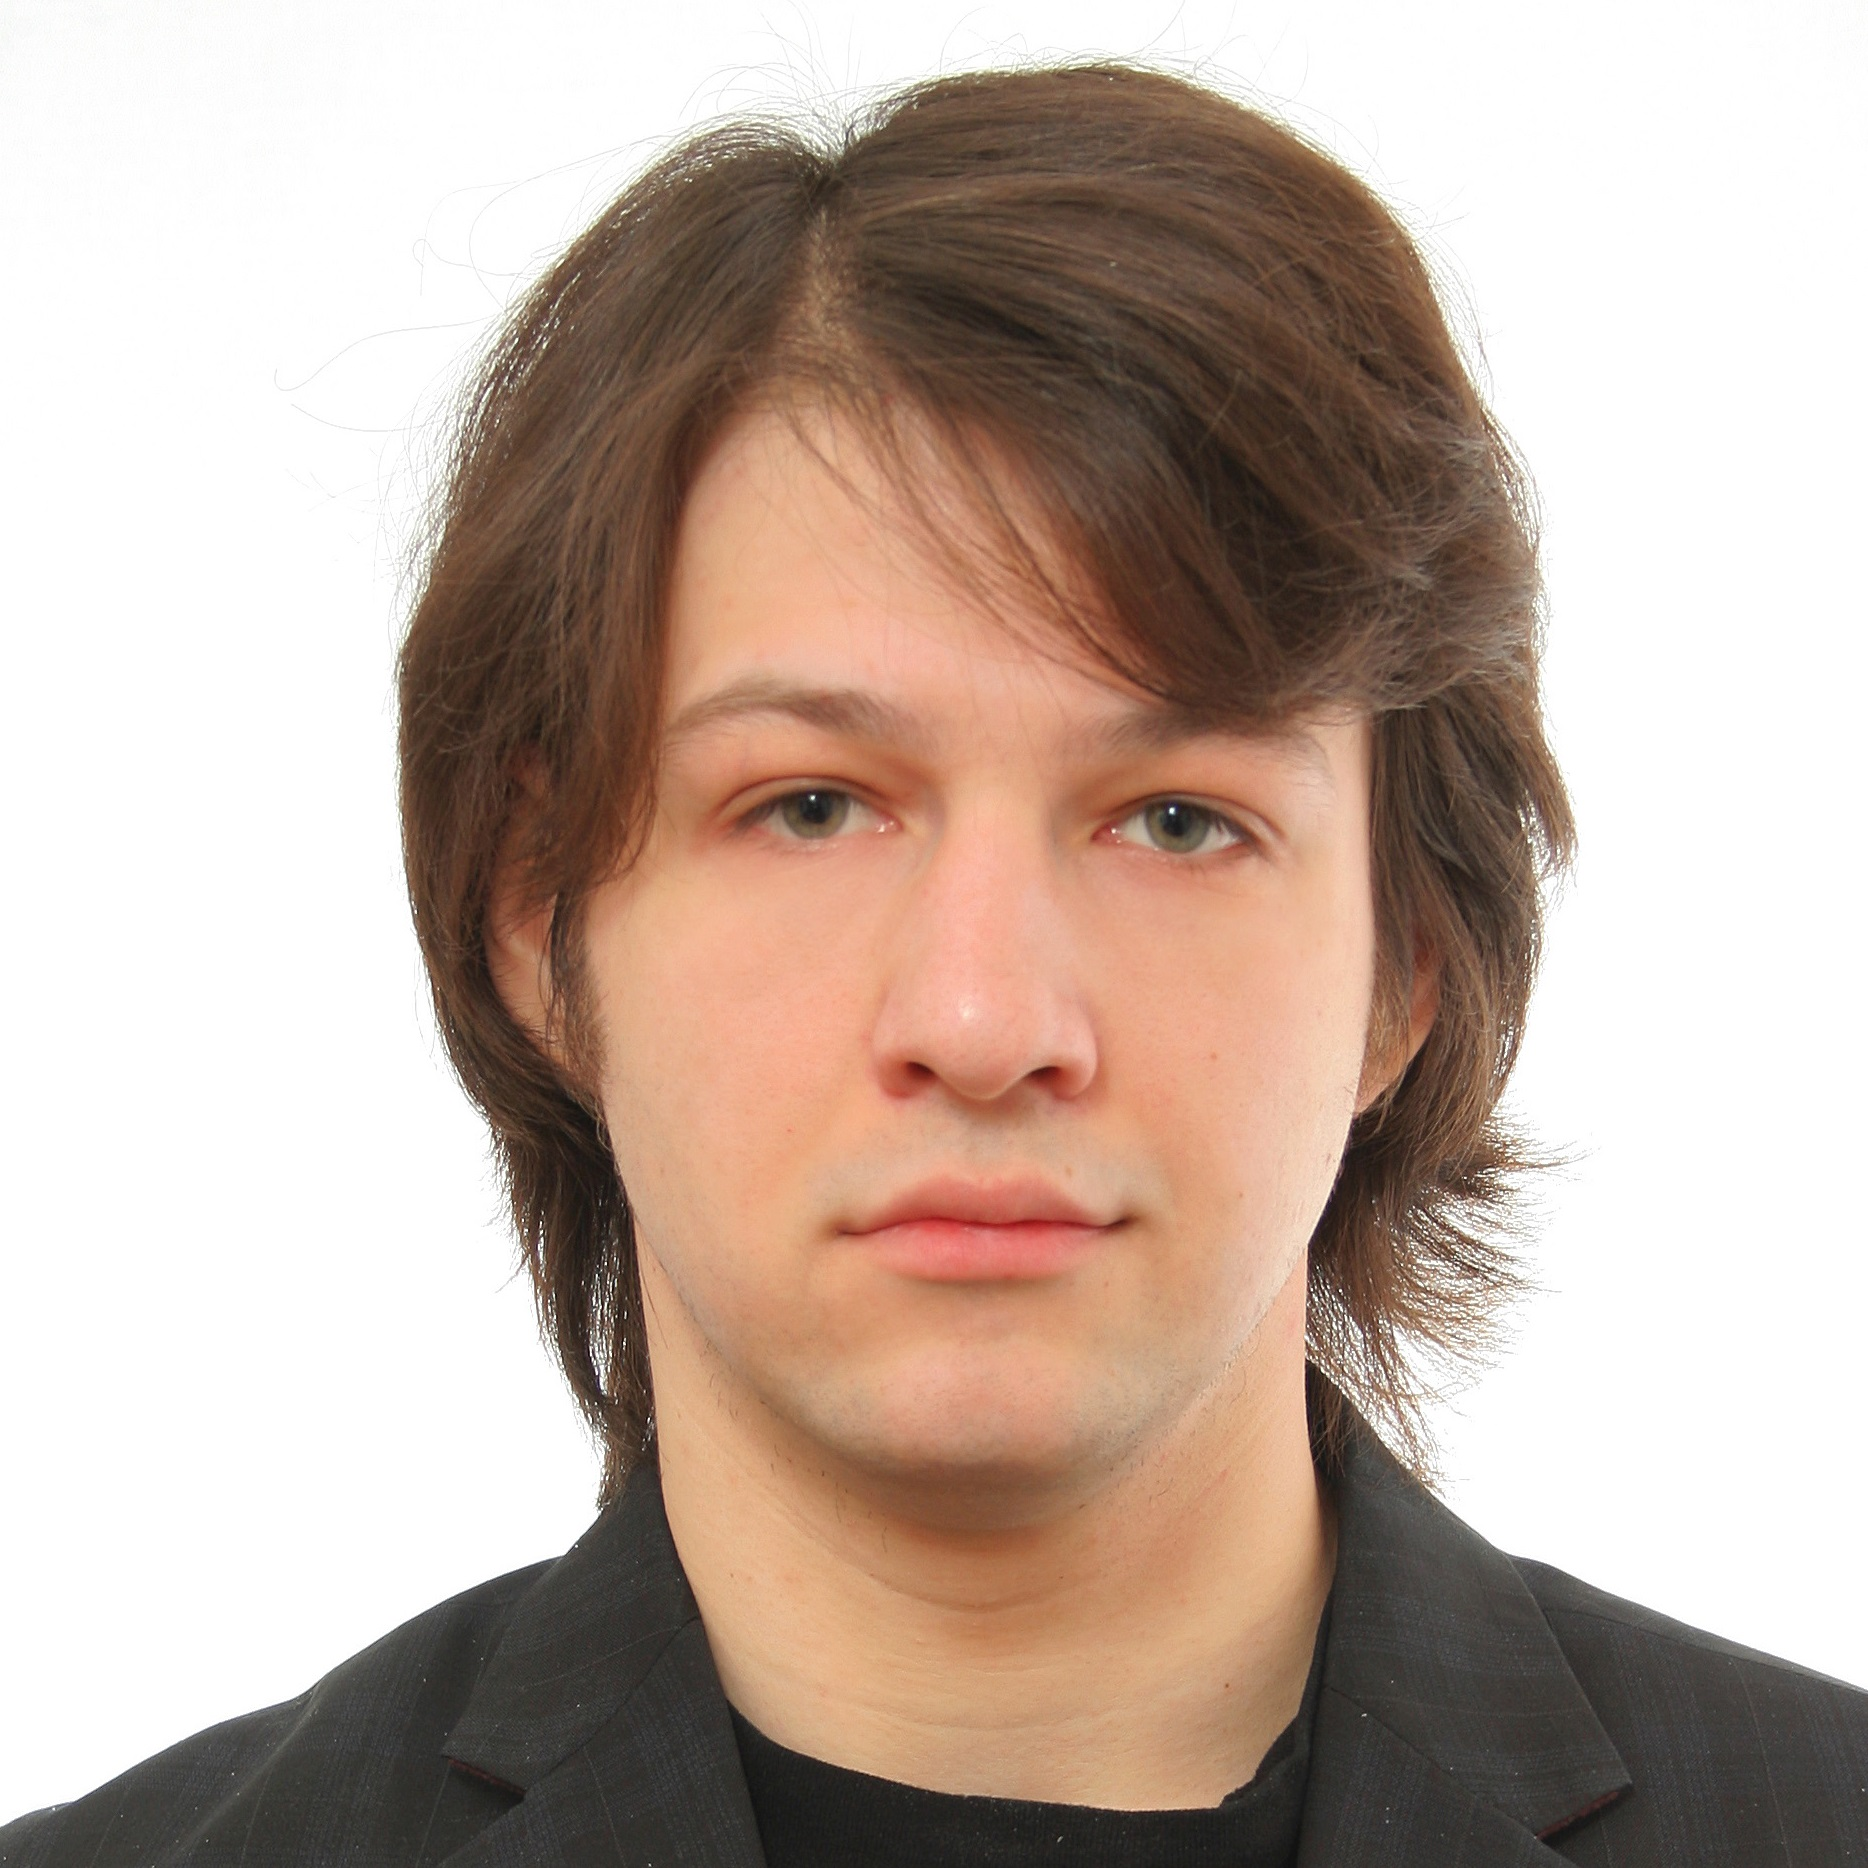
\includegraphics[height=12px]{./photo}
    \myurl{http://aakinshin.net}
}
\cvitem{GitHub}{
    
\includegraphics[height=12px]{github}
    \myurl{https://github.com/AndreyAkinshin}
}
\cvitem{StackOverflow}{
    
\includegraphics[height=12px]{stackoverflow}
    \myurl{http://stackoverflow.com/users/184842/AndreyAkinshin}
}
\cvitem{Хабрахабр}{
    
\includegraphics[height=12px]{habr}
    \myurl{http://habrahabr.ru/users/dreamwalker}
}
\cvitem{LinkedIn}{
    
\includegraphics[height=12px]{linkedin}
    \myurl{http://www.linkedin.com/in/AndreyAkinshin}
}
\cvitem{SlideShare}{
    
\includegraphics[height=12px]{slideshare}
    \myurl{http://www.slideshare.net/AndreyAkinshin}
}
\cvitem{Google Scholar}{
    
\includegraphics[height=12px]{google-scholar}
    \myurl{http://scholar.google.ru/citations?user=rYVl83IAAAAJ}
}

\end{document}